\section*{Exceptions}
Wenn eine Exception nirgendwo gecached wird und somit \texttt{main()} mit dieser Exception zurückkehrt, behandelt die JVM das mit einem Programmabbruch.
	\subsection*{Exception auslösen}
		Jede Funktion die entweder eine Exception auslöst oder eine allfällige Exception nicht behandelt, muss alle potentiellen Exceptions deklarieren, die der Aufrufer erhalten könnte.(ausnahme sind unchecked Exceptions)
		\lstinputlisting{code/Exception_throw.java}
	\subsection*{Exceptions behandeln}
		\lstinputlisting{code/Exception_catch.java}
	\subsection*{Exception Klassen}
		\begin{minipage}{9cm}
			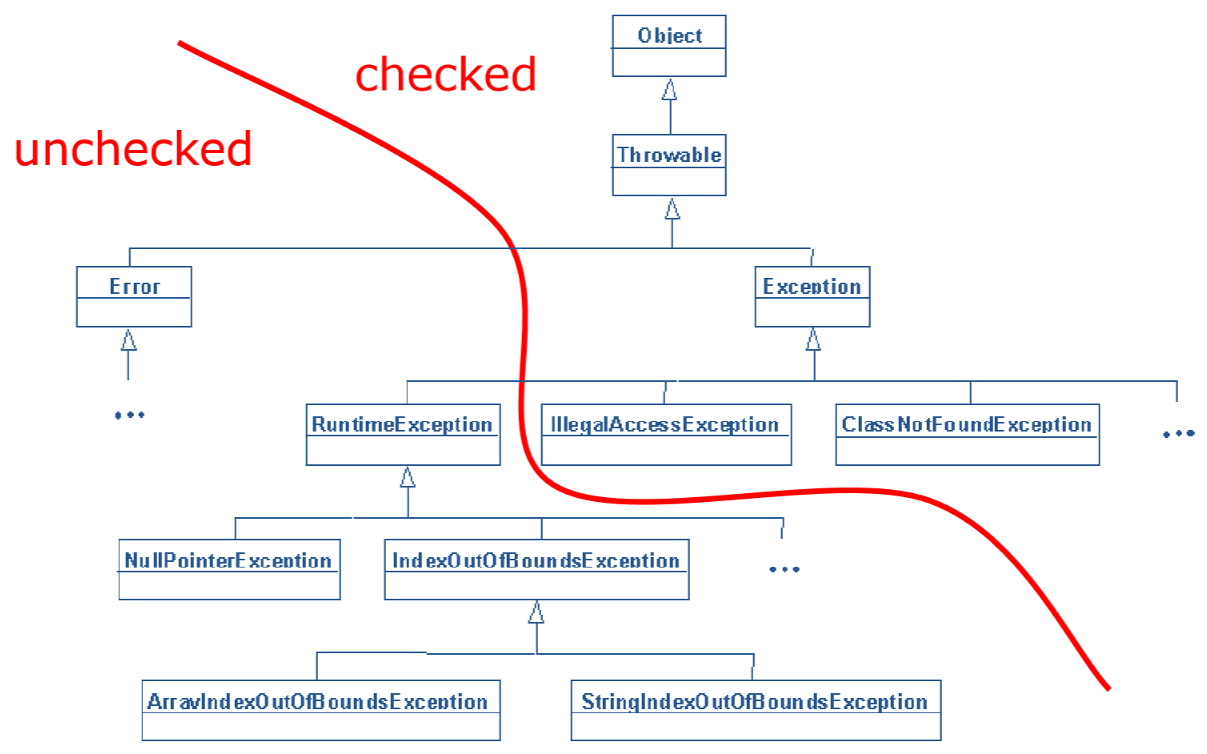
\includegraphics[width=\columnwidth]{pics/Exception_hierarchy.png}
		\end{minipage}
		\hspace*{0.5cm}
		\begin{minipage}{9.3cm}
			\textbf{Checked Exceptions:}\vspace{-0.2cm}
			\begin{itemize}[noitemsep]
				\item Exception muss behandelt werden, ODER
				\item throws-Deklaration in Methodenkopf.
				\item Vom Compiler geprüft
			\end{itemize}
			\textbf{Unchecked Exceptions:}\vspace*{-0.2cm}
			\begin{itemize}[noitemsep]
				\item Keine throws-Deklaration und keine Behandlung nötig
				\item kann aber behandelt werden, falls gewünscht
				\item \texttt{RuntimeExceptions} und \texttt{Error} sowie Unterklasen davon
				\item Nicht vom Compiler geprüft
			\end{itemize}
		\end{minipage}
	\subsection*{Benutzerdefinierte Exceptions}
		\lstinputlisting{code/Exception_own.java}
	\subsection*{Mehrere Catch-Klauseln}
		\begin{minipage}{8.5cm}
			\begin{itemize}[noitemsep]
				\item Passender Catch wird von oben nach unten gesucht
				\item Bei Exception wird \textbf{nur} der erste kompatible catch ausgeführt
				\item kein passendes Catch $\rightarrow$ Exception bleibt unbehandelt
			\end{itemize}
			\vspace*{0.5cm}
			\begin{itemize}[noitemsep]
				\item Wenn mehrere Exception Typen gleich behandelt werden sollen, ist ein sogenannter Multi-Catch möglich:
			\end{itemize}
		\end{minipage}
		\hspace{0.5cm}
		\begin{minipage}{9.8cm}
			\lstinputlisting{code/Exception_multiCatch.java}
			\lstinputlisting{code/Exception_multiCatch2.java}
		\end{minipage}
	\subsection*{finally-Block}
		\begin{itemize}[noitemsep]
			\item optionaler finally Block am Ende des try-Konstrukts.
			\item Wird in jedem Fall durchlaufen			
		\end{itemize}
		\begin{minipage}[t]{10cm}
			\lstinputlisting{code/Exception_finally.java}
		\end{minipage}
		\hspace*{0.5cm}
		\begin{minipage}[t]{7.3cm}
			\lstinputlisting{code/Exception_finallyWithoutCatch.java}
			$\rightarrow$ oftmals auch ohne \texttt{catch}-Block.
		\end{minipage}

		\begin{minipage}[t]{9cm}
			\lstinputlisting{code/Exception_finallyAuto.java}
			$\rightarrow$ Dieser Block ist äquivalent zum Block \textbf{rechts}, wobei der \texttt{finally}-Block automatisch vom Compiler generiert wird und um einiges komplexer ist. \textbf{Wichtig} dabei ist, dass in der Klasse \texttt{Scanner} das Interface \texttt{AutoCloseable} implementiert ist, damit dort die \texttt{close()}-Funktion sicher existiert. Mit \texttt{;}-getrennt können mehrere Variabeln definiert werden.
		\end{minipage}
		\hspace*{0.5cm}
		\begin{minipage}[t]{8.3cm}
			\lstinputlisting{code/Exception_finallyAuto2.java}
		\end{minipage}